% =====================================================================
%  多模态思维链推理综述 ——《计算机学报》双栏排版源码
%  说明：若本机已安装 cjc.cls，直接使用 \documentclass{cjc};
%       若无，则以 \documentclass[twocolumn]{ctexart} 等价替代。
% =====================================================================
\documentclass[twocolumn]{ctexart}
% \documentclass{cjc}   % 《计算机学报》官方文档类（如已安装可切换）
% 编译方式：xelatex -> xelatex（两轮）

% ---------------- 宏包引入 ----------------
\usepackage[a4paper,top=2.5cm,bottom=2.5cm,left=2.0cm,right=2.0cm,columnsep=0.8cm]{geometry}
                               % ctexart 已提供中文支持，无需再加载 ctex
\usepackage{amsmath,amssymb,amsfonts}   % 数学公式
\usepackage{graphicx}                   % 插图（XeLaTeX下自动选xdvipdfmx驱动）
\usepackage{booktabs}                   % 三线表
\usepackage{multirow}                   % 多行表
\usepackage{array}                      % 表格列控制
\usepackage{tabularx}                   % 自适应栏宽表格
\newcolumntype{Y}{>{\raggedright\arraybackslash}X}  % 左对齐自适应列
\usepackage{caption}                    % 图表标题
\usepackage{subcaption}                 % 子图
\usepackage{float}                      % 浮动体控制
\usepackage{xcolor}                     % 颜色
\usepackage{enumitem}                   % 列表
\usepackage{url}                        % 超链接
\usepackage{cite}                       % 参考文献
\usepackage{balance}                    % 末栏平衡

% ---------------- 字体与排版规范（对应模板字号） ----------------
% 题目：2号黑体；作者：3号仿宋；正文：5号宋体；一级标题4号黑体，二级5号黑体，三级5号宋体
\ctexset{
  section   = {format = \zihao{4}\heiti,  beforeskip = 1ex, afterskip = 0.6ex},
  subsection= {format = \zihao{5}\heiti,  beforeskip = 0.8ex, afterskip = 0.4ex},
  subsubsection = {format = \zihao{5}\songti\bfseries, beforeskip = 0.6ex, afterskip = 0.3ex}
}

% ---------------- 图表标题样式（小5号） ----------------
\captionsetup{font={small},labelsep=quad}
\captionsetup[table]{position=top}

% ---------------- 自定义命令 ----------------
\newcommand{\mcot}{MCoT}  % 多模态思维链缩写
\newcommand{\vqgan}{VQ-GAN}
\newcommand{\dvae}{dVAE}

% =====================================================================
\title{\zihao{2}\heiti 多模态思维链推理：从视觉词元化到开放词汇奠基的范式演进与未来挑战}
\author{\zihao{3}\fangsong 马福泉}
\date{}

\begin{document}

\twocolumn[
\begin{@twocolumnfalse}
\maketitle

% ---------------- 摘要 ----------------
\noindent\zihao{-5}\songti\textbf{摘要}\quad
多模态思维链（Multimodal Chain-of-Thought, \mcot{}）推理通过将大语言模型的逐步推理范式延伸至视觉模态，正在重塑模式识别从“小样本感知映射”向“大模型认知推理”的演进路径。本文系统综述了多模态思维链推理的研究脉络，并以“开放词汇感知提供空间语义奠基 $\rightarrow$ 视觉词元化将图像转化为离散序列 $\rightarrow$ 统一 Transformer 实现多模态思维链动态演进”的层次逻辑为主线，贯通开放词汇感知、视觉词元表征与多模态大模型三大主题。首先剖析单阶段端到端推理与两阶段解耦推理（解释生成+答案预测）的动机演进与交叉注意力流差异；继而探讨连续特征与离散视觉词元对 CoT 推理稳定性的影响，揭示“以图思考”的实现机理；随后归纳自我纠正、工具驱动与原生视觉想象等前沿范式。在 ScienceQA 基准上，两阶段解耦框架将小模型（$<$1B）准确率提升 16.51 个百分点。最后凝练逻辑幻觉级联阻断、细粒度词元动态解耦、轻量化自适应剪枝与具身闭环演进四个深度挑战。
\vspace{0.5ex}

\noindent\zihao{-5}\songti\textbf{关键词}\quad 多模态思维链；视觉词元化；开放词汇感知；多模态大模型；以图思考；逻辑幻觉


\vspace{1.5ex}
\end{@twocolumnfalse}
]

% =====================================================================
%  章节层级标签（1~7级核心章节）
% =====================================================================

\section{引言}\label{sec:intro}
模式识别的发展史可被视为一部“表征能力”与“推理能力”交替跃迁的编年史。以 AlexNet 在 ImageNet 上的突破为标志，传统模式识别长期锚定于封闭类别空间下的判别式映射，其本质是学习一个从高维视觉特征到有限离散标签的映射函数 $f:\mathcal{X}\rightarrow\mathcal{Y}$，其中 $\mathcal{Y}$ 的基数在训练与测试阶段保持一致。此一范式依赖精心标注的任务相关标准数据集，虽在封闭设定下性能长足进步，却存在两个结构性缺陷：其一，感知与认知的割裂——模型仅完成“是什么”的判别，无从回答“为什么”的推理；其二，类别封闭性导致的开放场景失效——面对陌生类别时模型缺乏将环境感受与先验知识融合以创造新概念的能力，呈现“高风险、低适用”的特征。与此同时，大语言模型基于 Transformer 自注意力机制，经海量文本习得语言的深层规律与上下文逻辑，并涌现出思维链（Chain-of-Thought, CoT）能力\cite{wei2022cot}——通过将复杂问题分解为逐步子问题依次求解以提升推理性能。然纯文本 CoT 存在“模态单一”与“认知缺失”两大局限：文字能描述物体，却难以描述物体间的物理关系，“文本描述$\ll$视觉信息”，如同“阅读没有插图的教科书”，缺乏视觉辅助会限制复杂知识的获取与推理能力。多模态思维链（Multimodal Chain-of-Thought, \mcot{}）\cite{zhang2023mcot} 正是在此背景下被提出：它将 CoT 的逐步推理范式延伸至视觉模态，以视觉特征作为推理锚点，使模型在生成推理链（Rationale）时获得更强的监督信号，从而弥合感知与认知之间的鸿沟。

\subsection{模式识别范式的认知转向}\label{sec:intro:shift}
人类认知过程表明，人脑能够将环境感受与知识信息融合，并根据需要创造新概念、完成认知闭环。此一差异深刻启示：模式识别的下一跃迁必然自“感知映射”走向“认知推理”。传统感知算法设计受限于封闭概念空间，在开放场景中无法完成对陌生类别的正确识别；而开放词汇视觉感知要求模型自海量图文对数据中学习视觉概念知识，并在实际开放场景中实现不限类别的视觉感知，其类别开放性与描述开放性为认知推理奠定了语义先验。当此一开放语义先验与大语言模型的逐步推理能力相交汇，模式识别即自静态标签映射转向动态语义理解与逻辑推理，其目标由“判别”升级为“可解释的推断”。

\subsection{多模态思维链的提出动机与核心优势}\label{sec:intro:motiv}
\mcot{} 的核心优势体现于三方面：其一，减少幻觉——视觉特征作为锚点，显著减少了小模型（$<$1B 参数）在推理过程中的编造行为，视觉证据为每一推理步提供可校验的外部约束；其二，加速收敛——多模态信息提供了更强的监督信号，加快了模型的训练收敛速度；其三，性能提升——所生成的推理链（Rationale）质量更高，从而在 ScienceQA 等基准上将最终答案准确率推至当时的最优水平\cite{zhang2023mcot}。需指出的是，此三优势并非无代价：视觉特征的引入不可避免地增加了序列长度与计算开销，且跨模态对齐的偏差极易在多步推理中级联放大，故 \mcot{} 的研究重心始终在“收益”与“开销/风险”之间寻求权衡。

\subsection{本文的横向融合架构与组织脉络}\label{sec:intro:outline}
本文并非孤立讨论多模态思维链，而是构建一条贯穿三大主题的层次逻辑主线：开放词汇感知提供空间语义奠基 $\rightarrow$ 视觉词元化将图像转化为离散序列 $\rightarrow$ 统一 Transformer 实现多模态思维链动态演进。其中，开放词汇感知为推理链的每一步提供“可溯源的视觉坐标”，解决“指代不明”与“视觉幻觉”；视觉词元化使图像得以进入自回归框架，支撑“以图思考”；二者最终在统一 Transformer 中交汇，驱动思维链的动态演进。如图~\ref{fig:roadmap}所示，相关技术自 2022 年文本 CoT 经 2023 年开放词汇奠基与视觉词元化、2024 年解耦多模态 CoT，演进至 2026 年的统一交织流式 CoT。本文余下部分组织如下：第~\ref{sec:background} 节梳理相关工作与背景基础；第~\ref{sec:taxonomy} 节剖析多模态思维链的分类学与核心架构；第~\ref{sec:vtoken} 节论述视觉词元表征的底层赋能；第~\ref{sec:hierarchy} 节论证关键技术的层次逻辑协同；第~\ref{sec:comparison} 节给出主要方法的定量对比；第~\ref{sec:challenge} 节凝练研究挑战与未来方向；第~\ref{sec:conclusion} 节作结。

\begin{figure}[t]
  \centering
  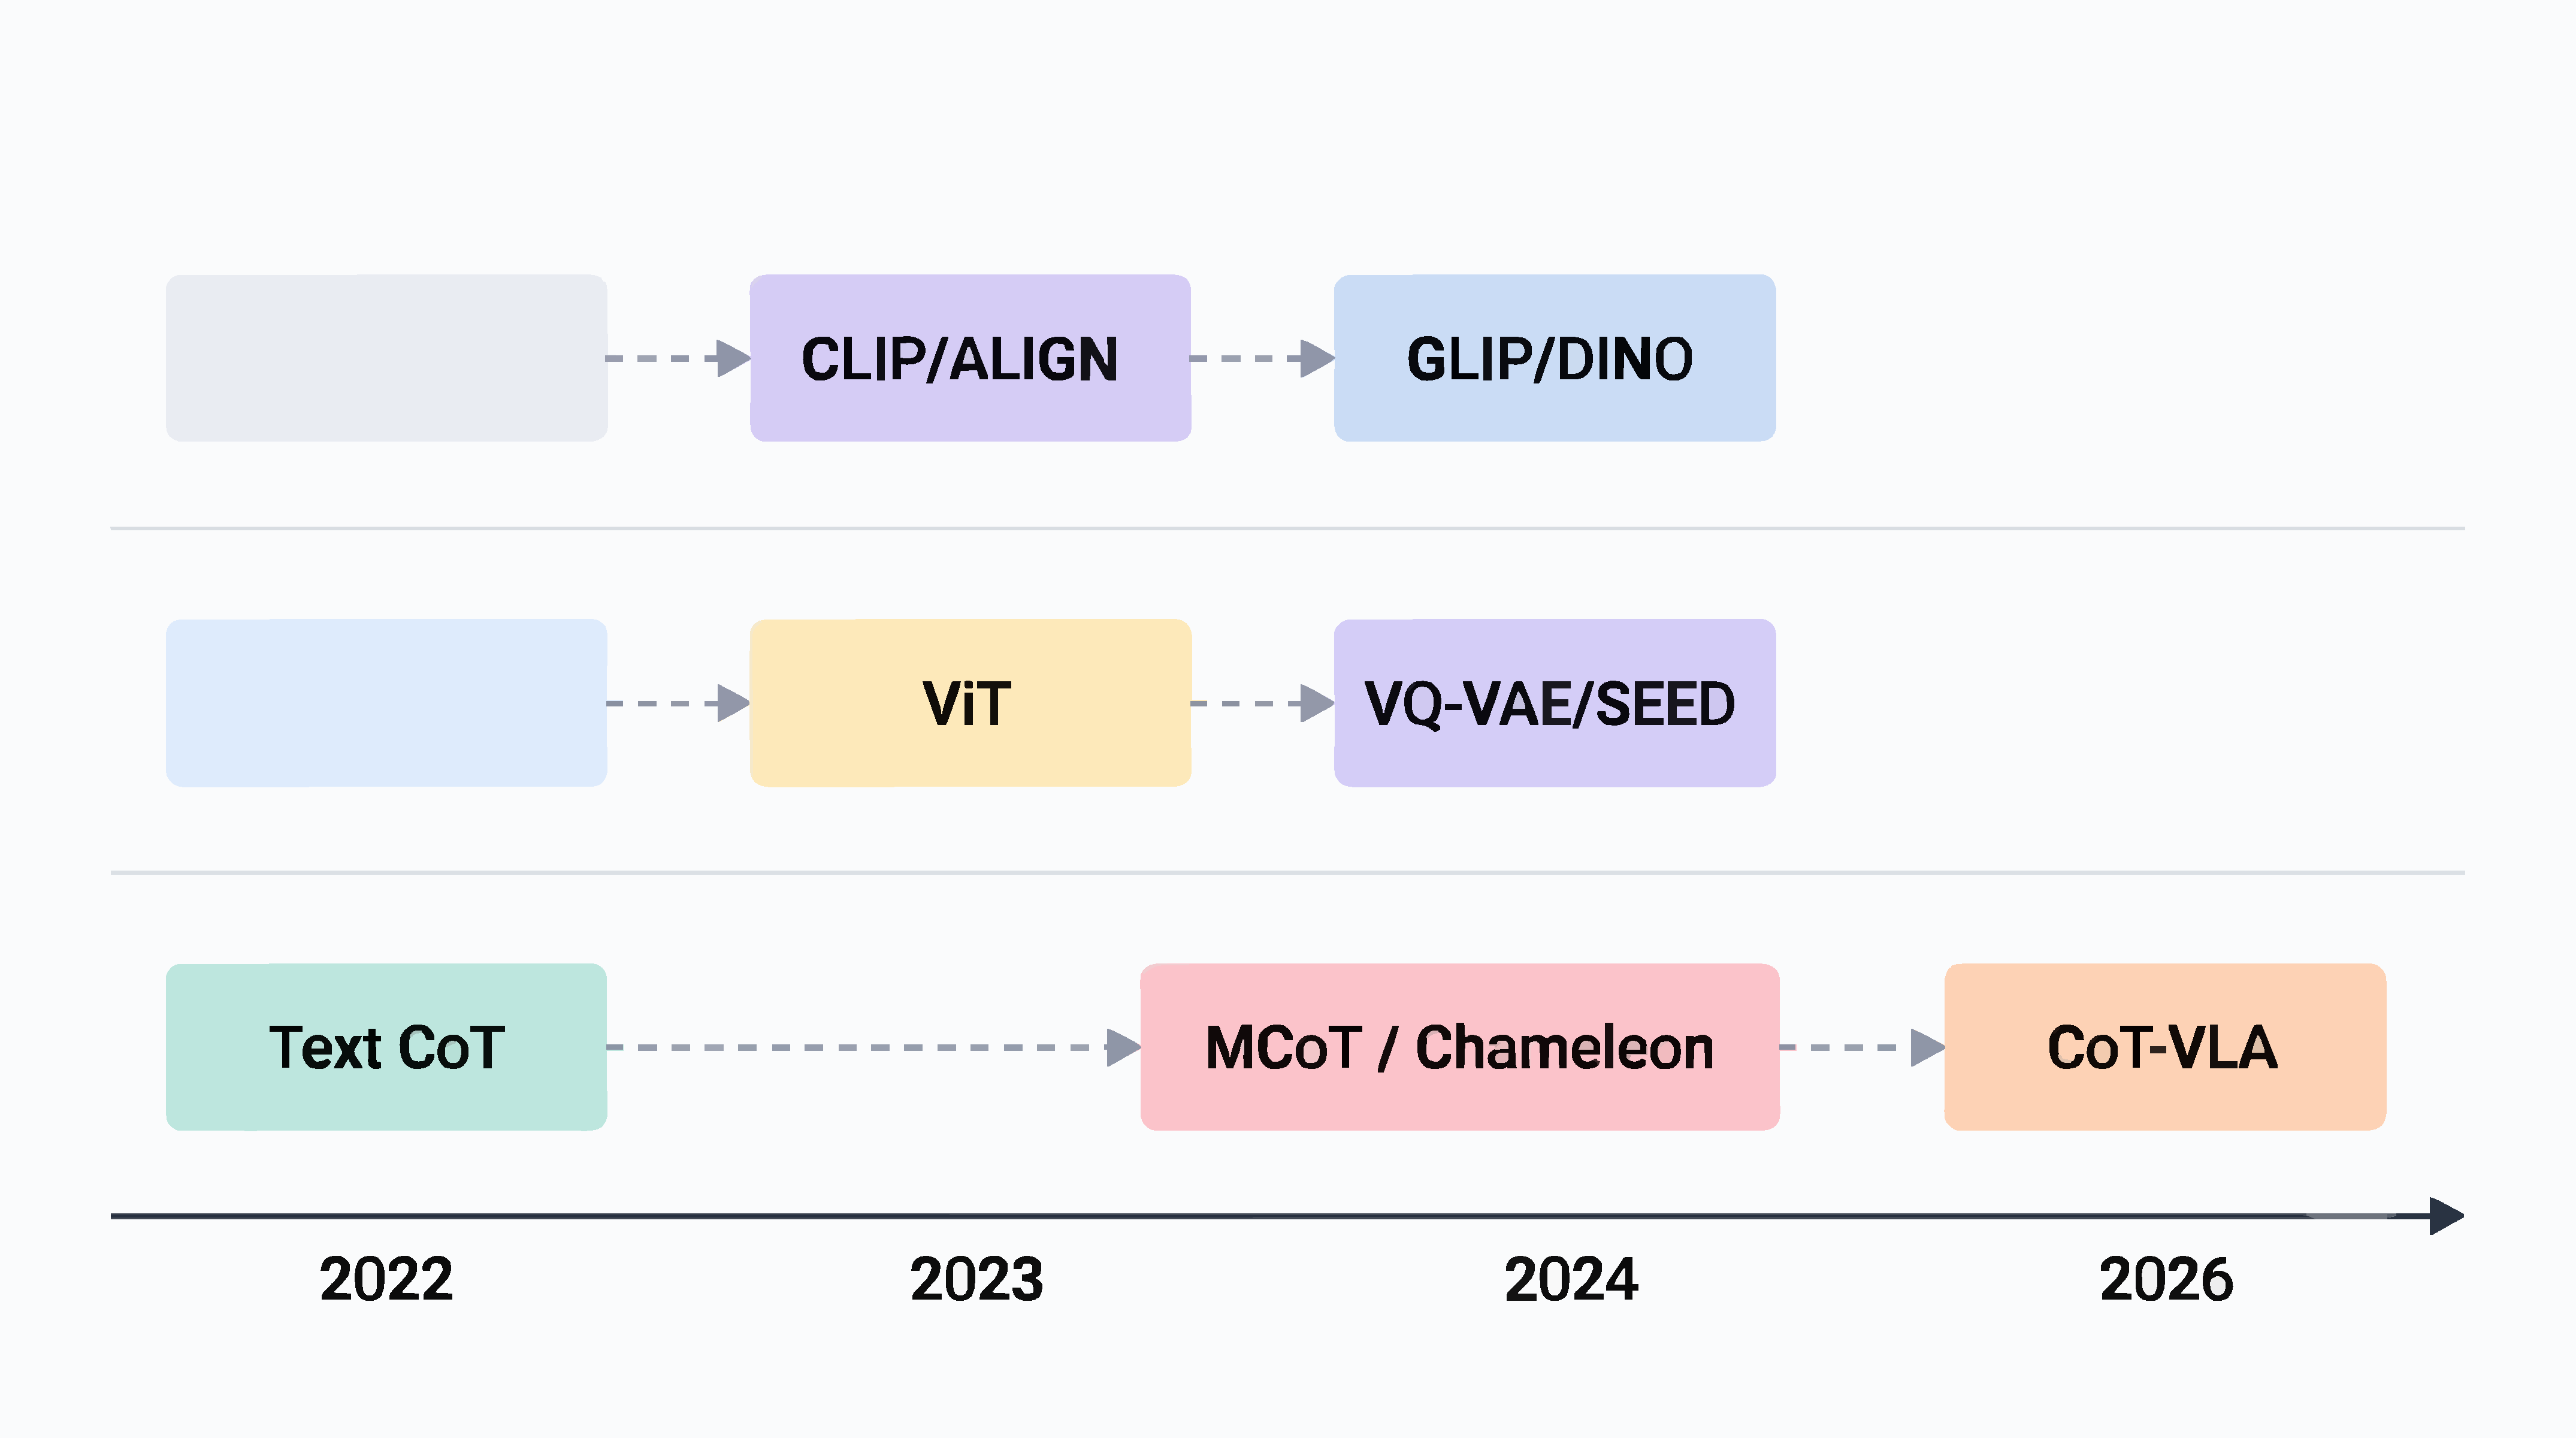
\includegraphics[width=\linewidth]{figs/fig1_roadmap}
  \caption{多模态思维链相关技术发展路线图归纳（自绘）。横向时间轴呈现自2022年至2026年相关技术的范式更迭与级联赋能过程。}\label{fig:roadmap}
\end{figure}

% =====================================================================
\section{相关工作与背景基础}\label{sec:background}
\subsection{大语言模型与思维链推理}\label{sec:bg:llm}
大语言模型（Large Language Model, LLM）是基于深度神经网络构建的先进人工智能系统，专门处理、理解和生成类人文本，其通过海量文本数据的训练掌握了语言的深层次规律与上下文逻辑。LLM 的核心架构基于 Transformer 系列网络，尤其是其中的自注意力机制——通过追踪序列数据中的关系以学习上下文及其含义。思维链（CoT）推理\cite{wei2022cot} 是 LLM 涌现的关键能力之一：通过让大模型逐步参与将复杂问题分解为一步一步的子问题并依次求解，可大幅提升推理性能，而这些推理的中间步骤即被称为思维链。CoT 与直接推理的根本差异在于，前者显式暴露了中间推理路径，使模型的“思考过程”可被观测、可被校验，亦为后续多模态扩展提供了结构化的载体。然纯文本 CoT 受限于语言模态的单调性，难以承载视觉等连续信号所蕴含的物理关系与空间结构，此即多模态思维链被提出的直接动因。

\subsection{视觉语言模型与多模态大模型}\label{sec:bg:vlm}
视觉语言模型（Vision-Language Model, VLM）通过将 LLM 与视觉编码器相结合构建多模态系统，使 LLM 具有"看"的能力。大多数 VLM 架构由三部分构成：视觉编码器（通常为基于 Transformer 的 CLIP 模型，已在数百万图文对上训练而具图文关联能力）、投影器（将视觉编码器输出转换为 LLM 可理解的图像标记，可为简单线性层或交叉注意力层）与 LLM 主干。LLaVA\cite{liu2024univl} 沿用 patchify 机制，以线性投影将 ViT 编码的连续视觉表征对齐至 LLM 嵌入空间。多模态大语言模型（Multimodal Large Language Model, MLLM）进一步扩展至文本、图像、视频、音频等全模态，其每种模态配备单独编码器，经融合模块将编码表示投影至统一嵌入空间。如图~\ref{fig:vlmarch}所示，VLM 的三部分架构与信息流向可被清晰刻画。须指出的是，MLLM 的推理计算复杂度除与序列长度呈二次方关系外，还需承担多模态编码与解码的额外开销，存在严峻的计算权衡。

\begin{figure}[t]
  \centering
  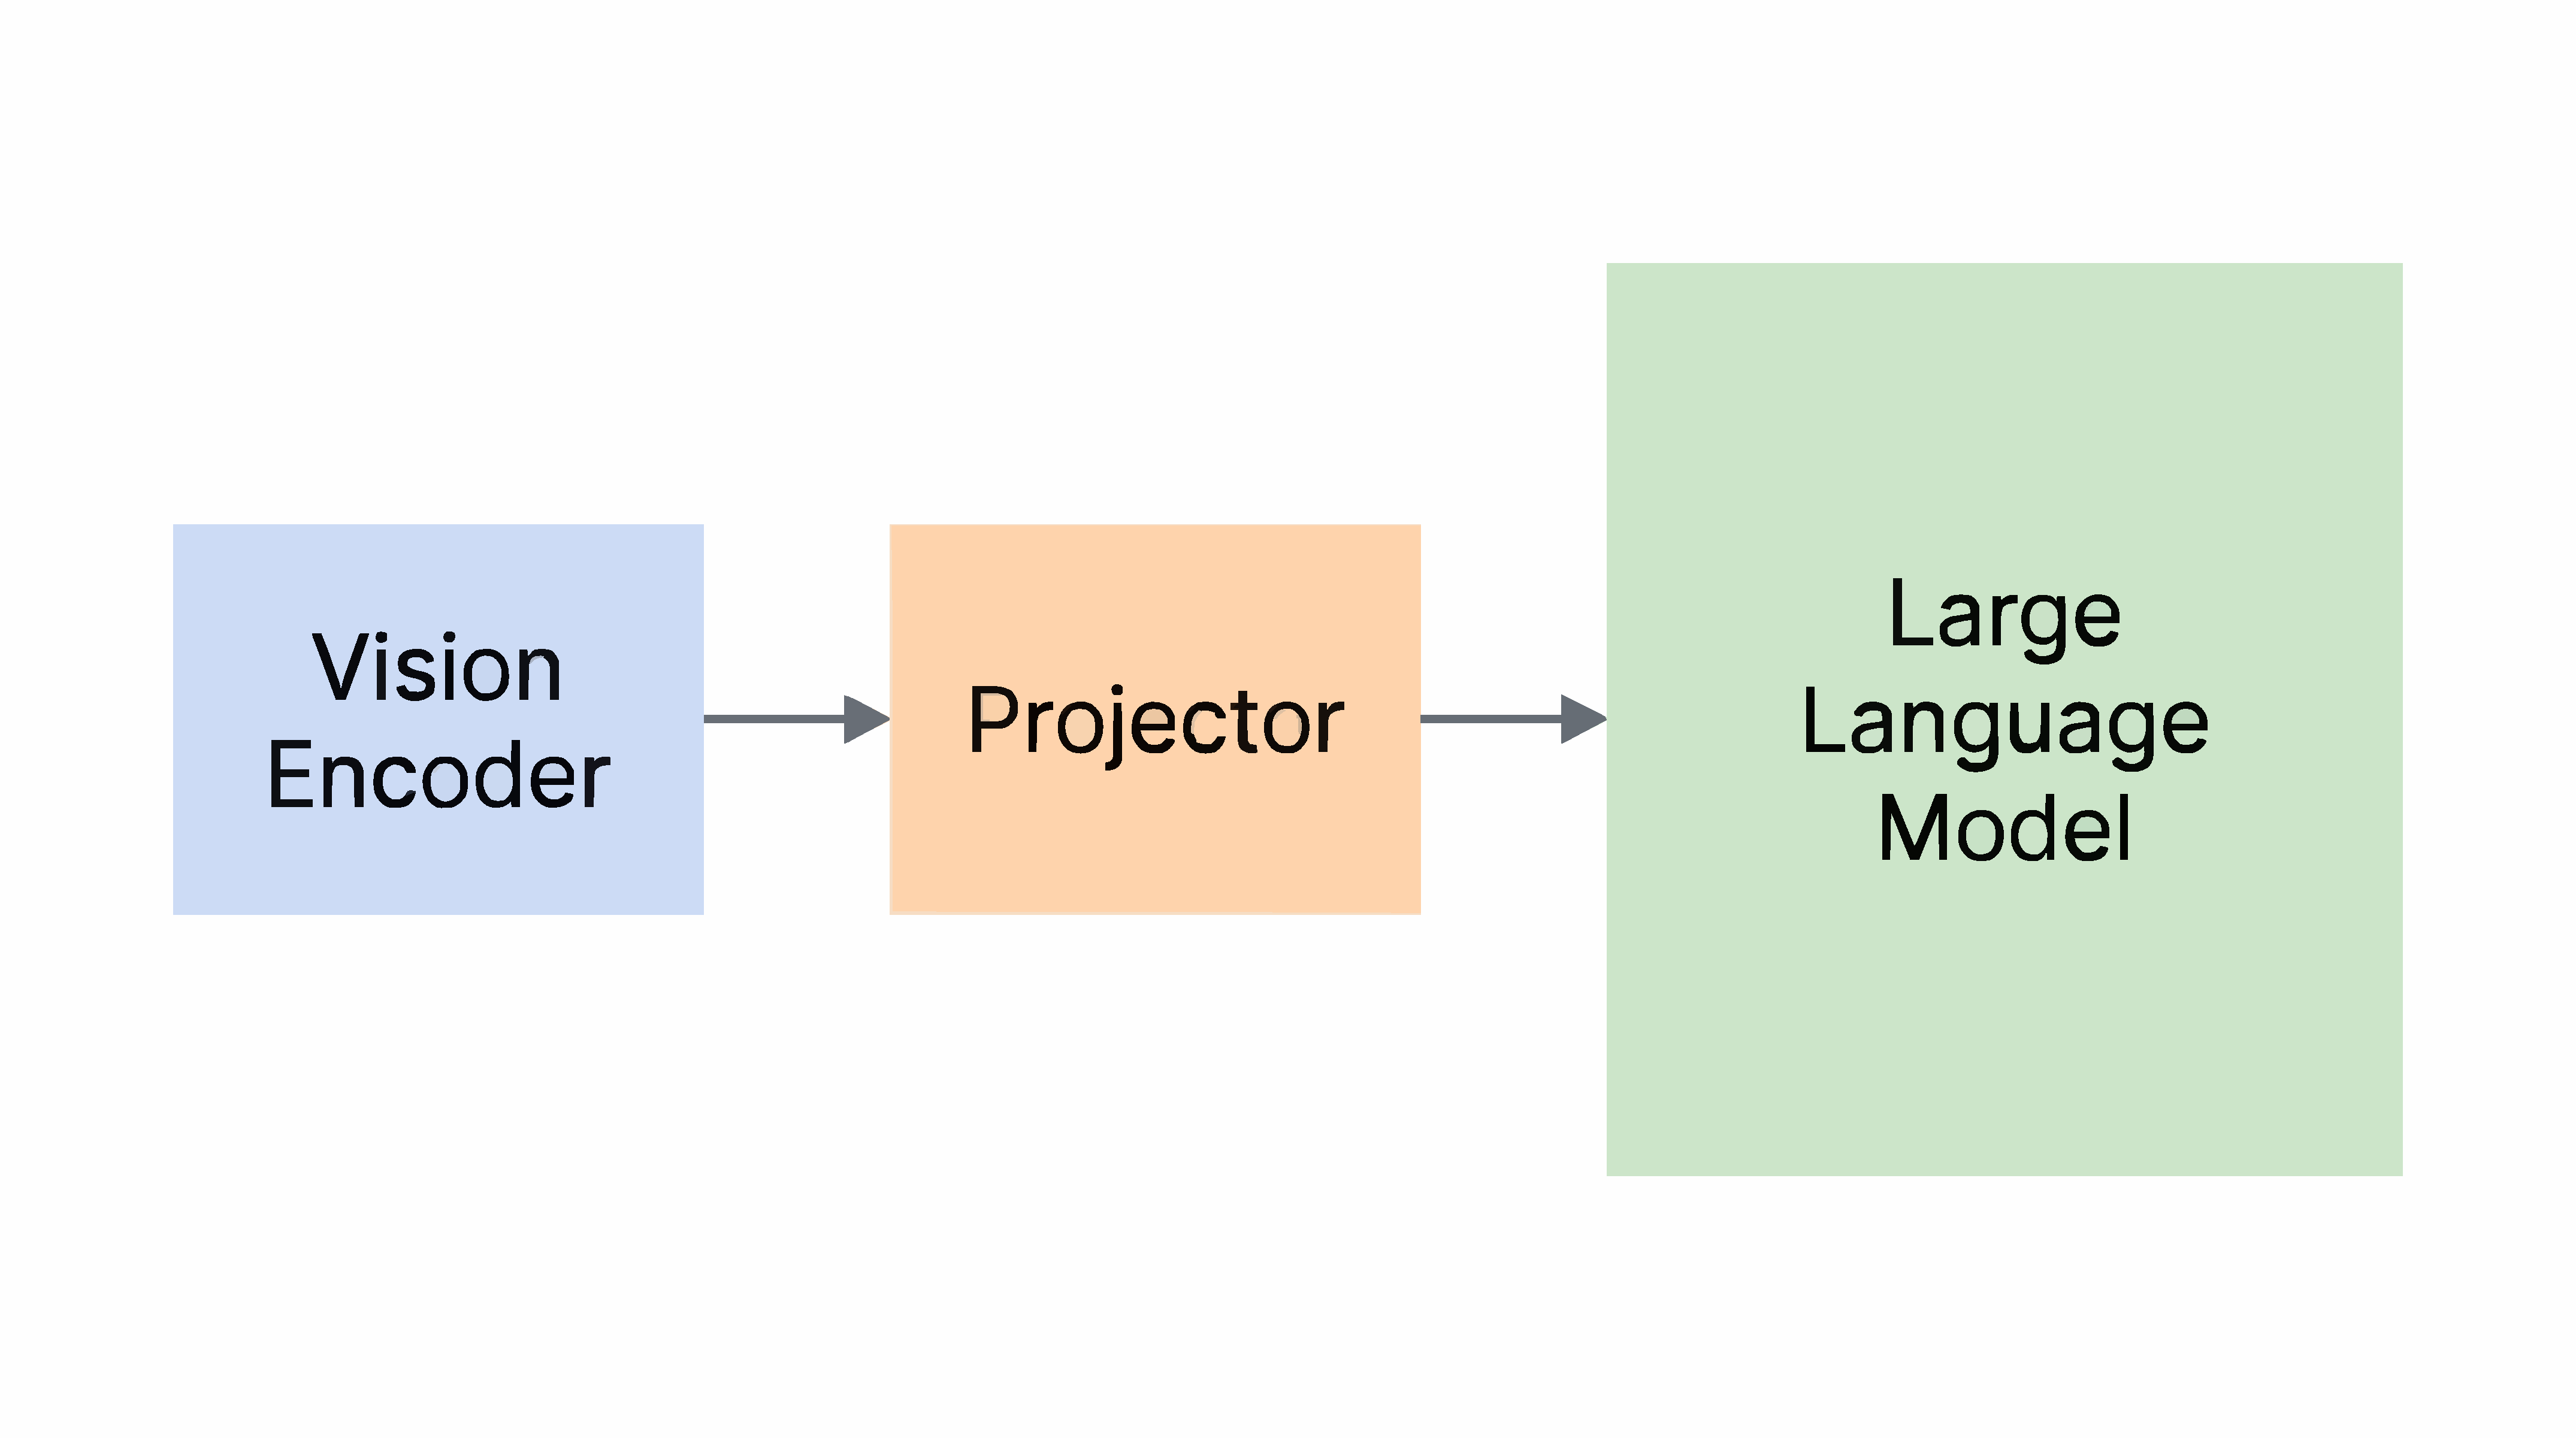
\includegraphics[width=\linewidth]{figs/fig_vlmarch}
  \caption{视觉语言模型的三部分通用架构（自绘）。包含视觉编码器（Vision Encoder）、投影器（Projector）与大语言模型（Large Language Model）三部分。}\label{fig:vlmarch}
\end{figure}

\subsection{开放词汇感知的语义奠基作用}\label{sec:bg:ovp}
开放词汇视觉感知要求模型自海量图文对数据中学习视觉概念知识，并在开放场景中实现不限类别的视觉感知，其类别开放性与描述开放性为多模态推理提供了语义先验。CLIP\cite{radford2021clip} 首个将 Transformer 与对比学习结合，自 4 亿互联网图文对训练多模态图文匹配模型，实现跨模态对齐与零样本预测能力；然 CLIP 的对齐仅及图像级，对边界框位置不敏感、区域识别率低。GLIP\cite{li2022gllip} 将物体检测与短语定位统一于区域-文本对比预训练，借助教师-学生半监督蒸馏自图文对构建区域-文本伪标签，使区域级语义奠基成为可能；Grounding-DINO\cite{liu2024groundingdino} 在特征编码、query 初始化与特征解码三层面注入细粒度多模态融合，支持指代表达理解。LISA\cite{li2023lisa} 则将奠基推向推理分割——通过在 LLM 词汇表中引入可学习的 $\langle\text{SEG}\rangle$ 词元，使模型得以输出需结合常识方能确定的分割区域。此一由图像级至区域级再至推理级的演进，为思维链中“指代什么”提供了可溯源的视觉坐标。

\subsection{视觉词元表征的离散化基础}\label{sec:bg:vtoken}
视觉词元化的首要问题是将二维图像转化为一维序列。ViT 将图像切分为固定大小的 patch，经展平与线性映射转化为 token 序列，并辅以位置编码以补偿空间结构信息的损失；然单一尺度 token 难以兼顾全局语义与局部细节，PVT、Swin Transformer 与 RegionViT 分别以多尺度金字塔、移位窗口与区域-局部注意力予以改进。真正使图像进入与文本同构离散空间的是 VQ-VAE\cite{van2017vqvae} 的向量量化：连续潜在特征经码本最近邻查找被替换为离散索引，图像由此被表达为有限词表上的离散序列。其生成变体 \vqgan{}\cite{esser2021vqgan} 以对抗训练与码本重构提升生成质量。SEED\cite{ge2023seed} 将受 2D 位置约束的 token 重构为适配左到右单向自注意力的因果序列，使 LLM 具备视觉理解与生成双重能力；UniTok\cite{fei2025unitok} 则以多码本量化（MCQ）弥合单码本难以兼顾细节重建与高层语义的缺陷。此一离散化基础，是后续“以图思考”中生成可操控视觉中间态的前提。

% =====================================================================
\section{多模态思维链的分类学与核心架构}\label{sec:taxonomy}
\subsection{两阶段解耦推理：解释生成与答案预测}\label{sec:tax:twostage}
% —— 核心数学公式（1）：两阶段概率分解 ——
\begin{equation}\label{eq:twostage}
P(a\mid I,Q)=\sum_{r}P_{\theta_{2}}(a\mid I,Q,r)\,P_{\theta_{1}}(r\mid I,Q)
\end{equation}
其中 $I$ 为图像，$Q$ 为问题，$r$ 为中间理由（Rationale），$\theta_{1},\theta_{2}$ 分别为两阶段模型参数。该解耦的动机在于将“理解（生成理由）”与“运用（预测答案）”分离，可分别对两阶段施加针对性监督，在小模型缺乏强先验时维持推理稳定性。其可解释性增益体现为：理由 $r$ 作为显式中间产物可被人工或自动校验，而非隐于黑盒之中。然误差累积是两阶段范式的固有风险——阶段一生成的理由若含谬误，将沿条件概率链级联放大至最终答案，此一信息瓶颈受限于阶段一的生成质量，故两阶段框架对理由生成的鲁棒性提出了远高于单阶段的要求。

\subsection{单阶段端到端推理与交织生成}\label{sec:tax:onstage}
为消解两阶段间的信息瓶颈，单阶段端到端推理以统一 Transformer 自回归地交织生成图文 token。Chameleon\cite{team2024chameleon} 采用混合模态早期融合，令视觉与文本 token 在每一层注意力中平等交互，不存在显式阶段划分。此一范式令跨模态对齐在底层即可建立，理论上有更优的跨模态一致性，然其对训练数据规模与模型容量提出更高要求——当模型容量不足时，缺乏阶段性监督的端到端交织反而易引发跨模态语义漂移，如表~\ref{tab:compare} 中 Chameleon 落后于两阶段框架所示。故单阶段并非两阶段的简单替代，而是以更高数据与算力开销换取表征一致性的另一权衡路径。

\subsection{交叉注意力流的对比分析}\label{sec:tax:crossattn}
两阶段与单阶段的本质差异在于跨模态信息的流动拓扑。两阶段解耦的交叉注意力流呈“接力式”：阶段一中视觉编码器与文本编码器经投影器对齐后，由交叉注意力将图像特征注入理由生成；理由作为桥接表征传递至阶段二，阶段二再次以交叉注意力融合“图+问题+理由”，其注意力流可刻画为 $\text{Attn}(Q_{\text{txt}},K_{\text{img}}\oplus K_{\text{rat}},V_{\text{img}}\oplus V_{\text{rat}})$，理由充当两阶段间的信息瓶颈，既是结构化监督之优势亦是信息压缩损失之风险。单阶段交织的交叉注意力流呈“网状式”：所有模态 token 共享同一注意力空间，视觉与文本在每一层双向交互，不存在显式瓶颈，此一“早期融合”使跨模态对齐在底层建立，但牺牲了阶段性可解释性。如图~\ref{fig:twostage}所示，两阶段架构中理由 $r$ 的瓶颈位置被显式标出。

\begin{figure}[t]
  \centering
  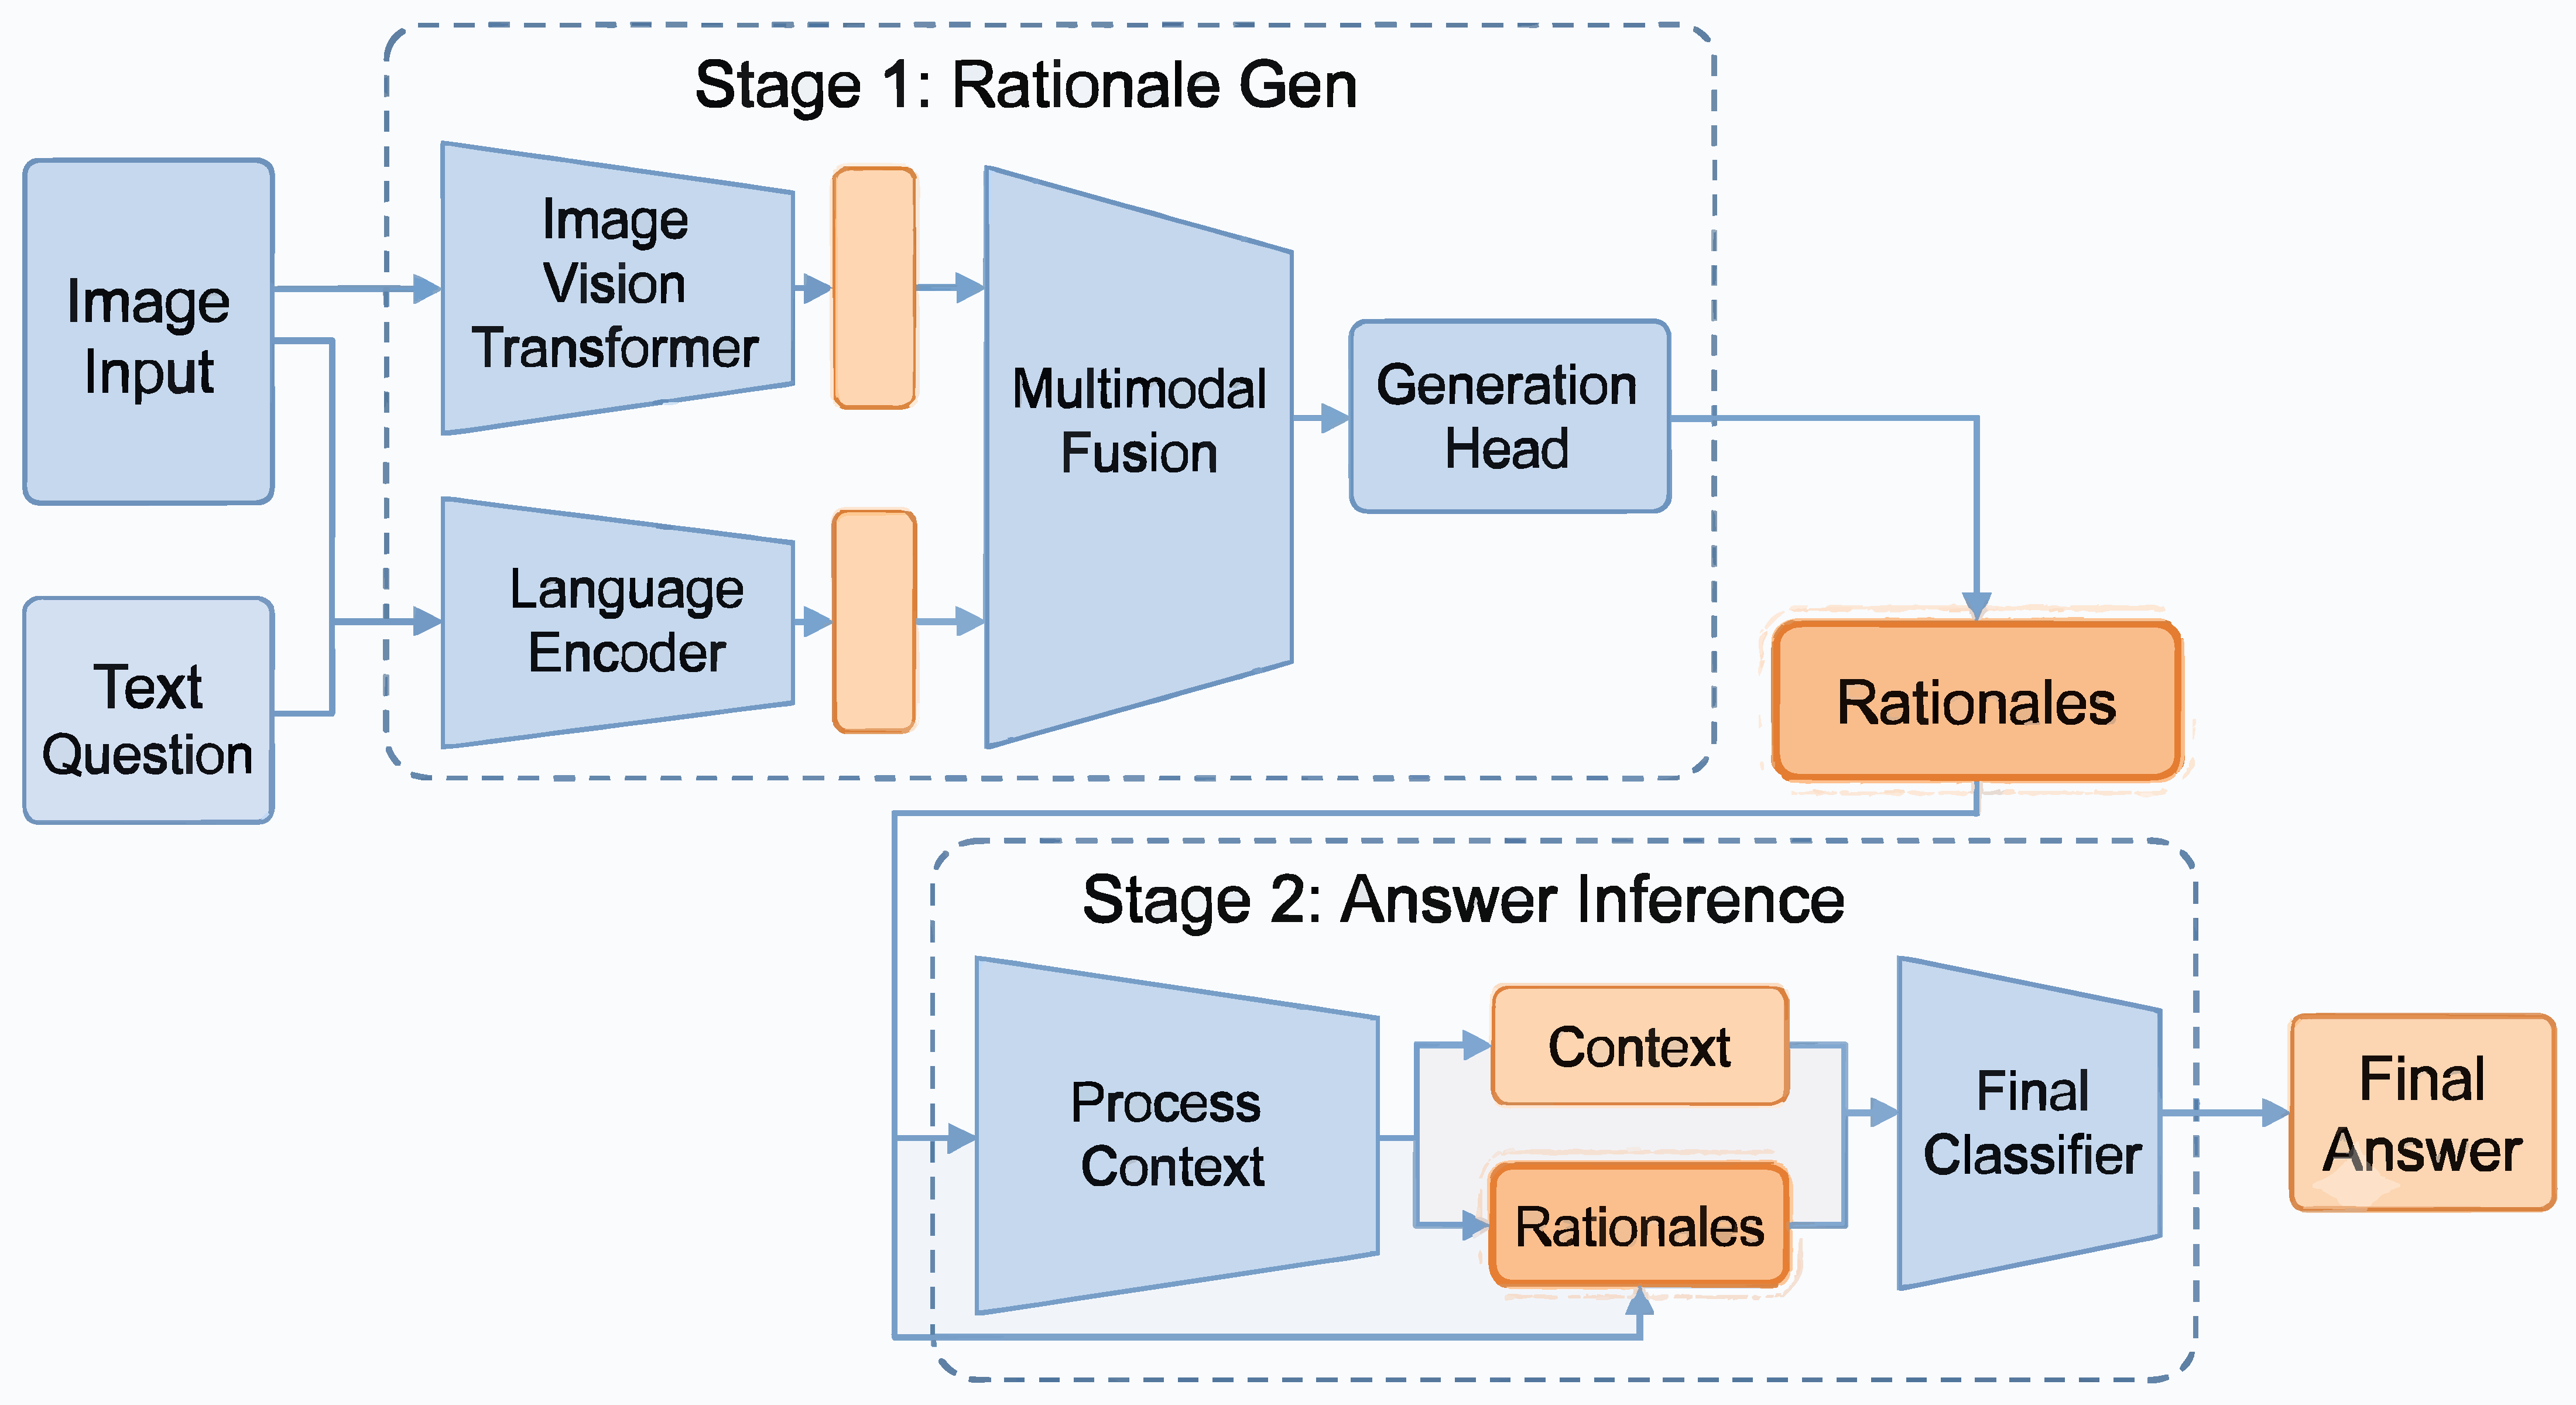
\includegraphics[width=\linewidth]{figs/fig2_twostage}
  \caption{双阶段解耦式多模态思维链核心架构图（自绘）。左侧输入经阶段一（Stage 1）生成中间推理步骤，再联合送入阶段二（Stage 2）预测最终答案。}\label{fig:twostage}
\end{figure}

\subsection{自我纠正与反思机制}\label{sec:tax:selfcorrect}
针对“想错了怎么办”，多模态思维链衍生出两大流派。事后特征验证流派以 Woodpecker 为代表，采用“做完再检查”策略，经关键概念提取、问题构建、视觉知识验证与视觉主张生成四步构建针对图像的特定视觉知识库，以边界框为证据修正响应中的幻觉，专治“看错”（视觉幻觉：无中生有、数错个数、属性标错）。动态反思架构流派则采用“边做边改”策略：Self-Refine 基于反馈迭代定位问题并完善答案，Self-Review 先评估答案正误、正确则保留、错误则调用 Self-Refine 改进，Self-Choose 对比多条推理路径择优或综合生成更佳答案，专治“想错”（逻辑谬误：公式用错、前后矛盾、推理断层）。两流派的核心差异可由表~\ref{tab:selfcorrect}系统对比。两流派分别适用于密集图像描述、医疗影像诊断（对事实准确度要求极高）与数学几何解题、复杂图表分析（对逻辑严密性要求极高）之场景，然二者均不可避免地引入了额外的判别开销，且反思过程本身亦可能产生新的谬误。

\begin{table}[htbp]
  \centering
  \caption{多模态思维链自我纠正两流派对比}\label{tab:selfcorrect}
  \small
  \begin{tabularx}{\linewidth}{lYY}
    \toprule
    维度 & 事后特征验证 & 动态反思架构 \\
    \midrule
    代表方法 & Woodpecker & Self-Refine等 \\
    核心思想 & 做完再检查 & 边做边改 \\
    纠错时机 & 事后Post-hoc & 推演中In-process \\
    纠错重点 & 视觉幻觉(看错) & 逻辑谬误(想错) \\
    运作机制 & 实体提取$\to$回溯 & 多分支择优 \\
    适用场景 & 密集描述、医疗 & 几何解题、图表 \\
    \bottomrule
  \end{tabularx}
\end{table}

% =====================================================================
\section{视觉词元表征对多模态推理的底层赋能}\label{sec:vtoken}

\subsection{从连续特征到离散视觉词元的范式跃迁}\label{sec:vt:contdisc}
以 LLaVA\cite{liu2024univl} 为代表的主流视觉语言模型沿用 patchify 机制，图像经 ViT 编码后由一个可训练的线性投影层将连续视觉表征强行对齐至 LLM 的词嵌入空间。该连续嵌入路径虽在端到端梯度反传上较为便利，却不可避免地引入了噪声与表征失稳：CLIP\cite{radford2021clip} 提取的连续向量处于一个高维且未加离散约束的流形之上，其几何结构受限于对比学习的对齐目标，难以保证在多步 CoT 推理过程中维持逐级的语义一致性。具体而言，当推理链跨越多个自回归步时，连续特征所携带的细粒度视觉证据被反复经由注意力机制重加权与再分配，存在严峻的计算权衡（trade-off）——表征分辨率越高则序列越长、$O(N^{2})$ 的自注意力开销越大，而一旦为妥协于硬件开销而过度压缩 token 数量，又极易导致表征坍塌，使得前序步骤所锚定的视觉细节在后序步骤中被注意力稀释乃至遗忘，引发跨模态语义漂移（semantic drift）。换言之，连续嵌入在多步推理中的“失忆”与累积误差，其根源在于缺乏一种离散的、可索引的、与文本词元同构的中间状态以供逐步校验。

相对地，以 VQ-VAE\cite{van2017vqvae} 及其生成变体 \vqgan{}\cite{esser2021vqgan} 为代表的向量量化路径，通过将连续潜在特征映射至一个有限且可学习的码本（codebook）实现离散化。向量量化的离散化过程可由如下目标函数刻画，其中编码器 $E$、解码器 $D$ 与码本 $\mathcal{Z}=\{z_k\}_{k=1}^{K}$ 联合优化，$\text{sg}(\cdot)$ 为停止梯度算子：
\begin{multline}\label{eq:vq}
\mathcal{L}_{\text{VQ}}=\|x-D(\text{sg}(z_{q}))\|_{2}^{2}+\|z_{e}-\text{sg}(z_{q})\|_{2}^{2} \\
+\,\beta\|\text{sg}(z_{e})-z_{q}\|_{2}^{2}
\end{multline}
其中 $z_{e}=E(x)$ 为连续潜在特征，$z_{q}=\arg\min_{z_k\in\mathcal{Z}}\|z_{e}-z_k\|$ 为码本最近邻量化结果。第一项为重构损失，第二项将码本向量拉向编码器输出（codebook loss），第三项将编码器输出拉向码本向量（commitment loss），$\beta$ 为权衡系数。该三损失项的耦合表明，离散化本质上是重构保真度与码本约束之间的折中——过强的 commitment 会令表征坍塌于少数码字，过弱则令码本游离于编码器流形之外，此即码本坍塌（codebook collapse）的数学根源。每一个图像块经编码器映射为连续向量后，在码本中执行最近邻查找并被替换为对应的离散索引，由此图像被转化为一个由离散视觉词元构成的序列。这一离散化虽以有损量化为代价，却在结构上与 LLM 最擅长的离散词元 next-token prediction 范式天然契合：离散词元为推理链提供了可生成、可插值、可显式溯源的中间状态，每一推理步所引用的视觉证据均可被回溯至码本中的确定索引，从而为阻断逻辑幻觉奠定了可校验的离散基座。然而需指出的是，UniTok\cite{fei2025unitok} 的消融实验揭示，将 768 维特征压缩至 16 维再量化入仅含 $16\text{k}$ 项的码本会造成 VQA 性能的不可忽视的衰减，单码本难以同时兼顾细节重建与高层语义。为此，SEED\cite{ge2023seed} 将受 2D 物理块位置约束的 token 重构为适配左到右单向自注意力的因果序列，而 UniTok 所提出的多码本量化（Multi-Codebook Quantization, MCQ）将长向量切分为若干子块各自量化，以多级码本弥合离散化损失。上述改进表明，离散视觉词元与文本词元表征空间的对齐并非简单的维度匹配，而是一个需要在量化分辨率、码本容量与自回归因果性之间反复折中的工程命题。

\subsection{“以图思考”的自回归演进机制}\label{sec:vt:thinking}
当离散视觉词元与文本词元共享同一自回归框架后，推理链不再被约束于纯语言模态，模型得以在中间步骤不仅预测下一个文本词元，还可自回归地预测下一个视觉词元，此即“以图思考”的数学实质。设推理序列为图文交织的混合词元流 $s_{1:T}=(s_{1},s_{2},\dots,s_{T})$，其中每个 $s_{t}$ 既可能来自文本词表 $\mathcal{V}_{\text{txt}}$ 亦可能来自视觉码本 $\mathcal{V}_{\text{vis}}$，则联合概率分布可被分解为：
\begin{multline}\label{eq:thinking}
P(s_{1:T}\mid I_{0},Q)=\prod_{t=1}^{T}P_{\theta}\!\bigl(s_{t}\mid I_{t},Q,\{s_{<t}\}\bigr), \\
I_{t}=\mathcal{T}_{t}\!\bigl(I_{0},\hat{s}_{<t}\bigr)
\end{multline}
其中 $\mathcal{T}_{t}$ 表示第 $t$ 步依据已生成词元 $\hat{s}_{<t}$ 对原始图像 $I_{0}$ 施加的视觉操作（如裁剪、缩放、Set-of-Mark 标注）；当 $s_{t}\in\mathcal{V}_{\text{vis}}$ 时，模型自回归地预测下一个视觉词元以更新中间图像状态 $I_{t}$，当 $s_{t}\in\mathcal{V}_{\text{txt}}$ 时则延续语言推理。该机制使图像从推理前的静态固定序列转变为可被逐步改写的"草稿"。此类工具驱动范式受限于预设工具集的表达边界，Visual Planning\cite{xu2026visualplanning} 则走至极端——仅以图像作为推理模态、以 GRPO 策略初始化生成合法图像轨迹。如图~\ref{fig:thinking}所示，"以图思考"自固定工具集经程序化操作至原生视觉想象的演进可被概括为视觉操作算子 $\mathcal{T}_{t}$ 表达能力的逐级释放，但随之而来的图文模态一致性与物理约束缺失问题仍悬而未决。

\begin{figure*}[t]
  \centering
  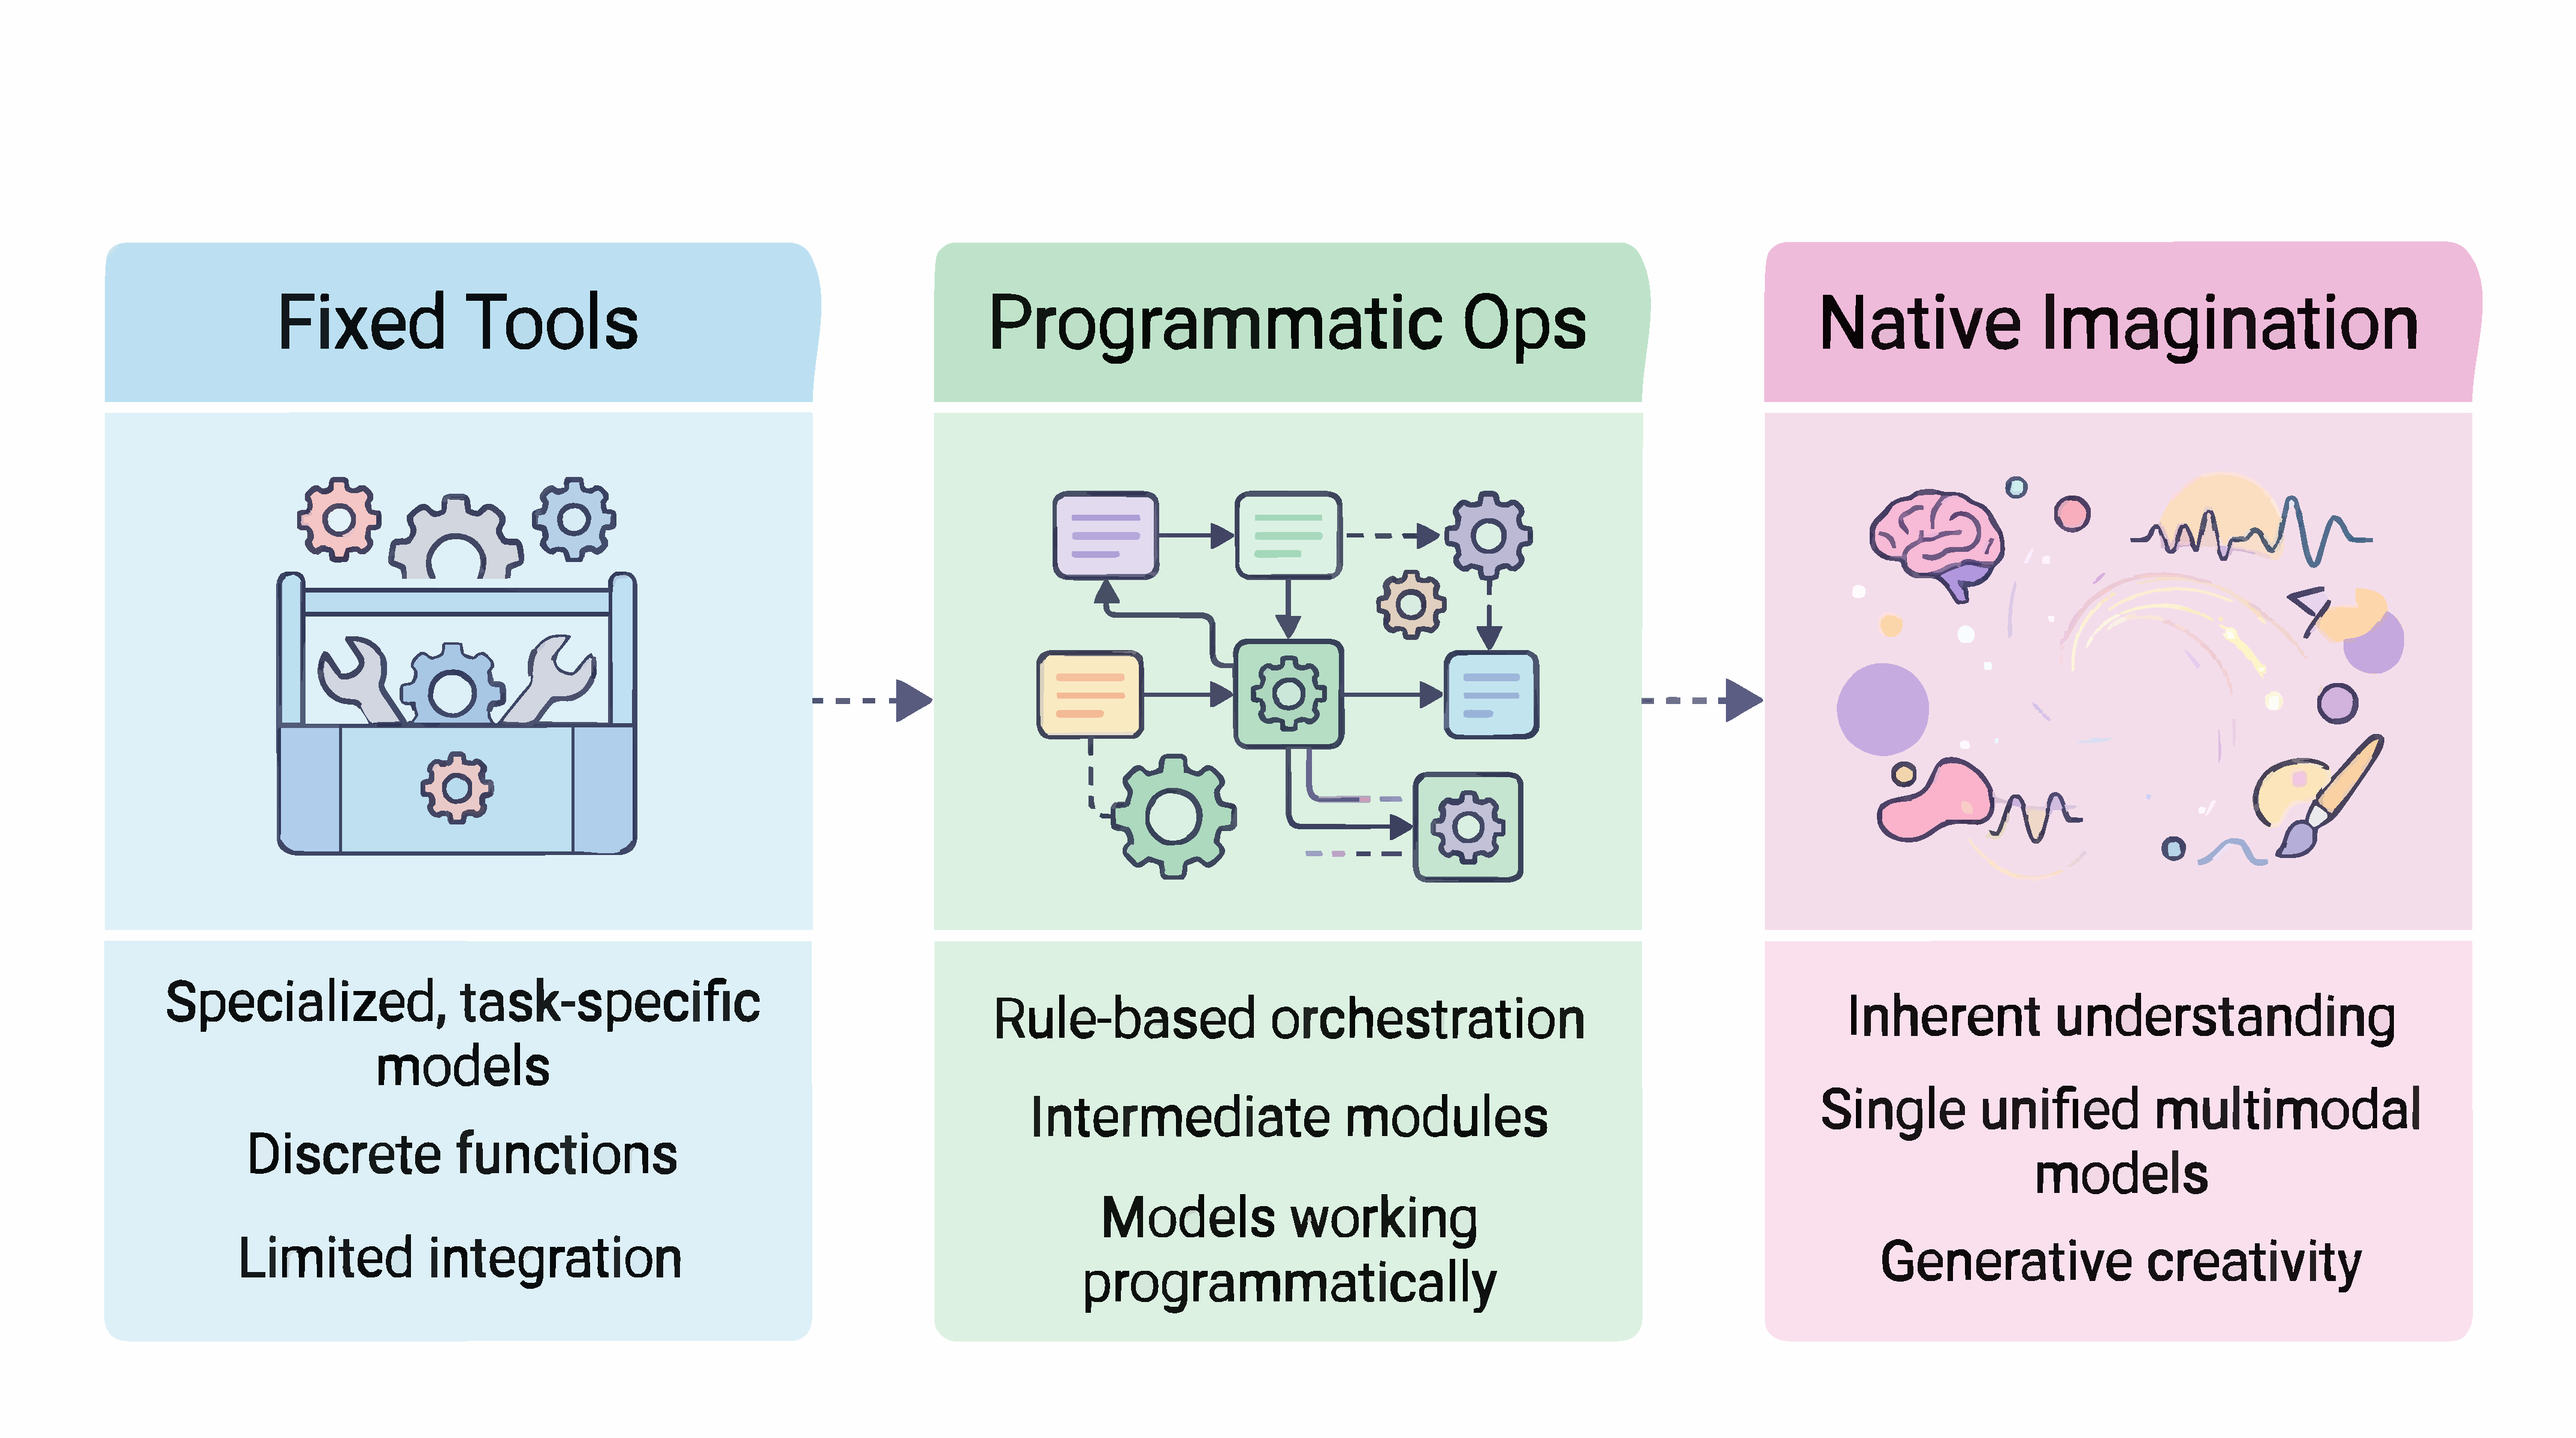
\includegraphics[width=0.85\textwidth]{figs/fig_thinking}
  \caption{“以图思考”三阶段演进示意（自绘）。自固定工具集（Fixed Tools）经程序化操作（Programmatic Ops）至原生视觉想象（Native Imagination），模型对图像的操作能力逐级增强。}\label{fig:thinking}
\end{figure*}

\subsection{统一词元建模与原生视觉想象}\label{sec:vt:unified}
原生视觉想象要求模型生成中间图像作为思考过程，这进一步将统一词元建模推向具身闭环。CoT-VLA\cite{zhao2025cotvla} 预测未来下一帧图像作为子目标、再据此生成机器人动作，FutureSightDrive\cite{zhang2025fsd} 以时空 CoT 同时预测未来帧、车道线与 3D 检测框以约束自动驾驶轨迹。此类工作表明，当视觉词元的生成与文本词元的推理在统一 Transformer 内交织时，思维链已从“语言独白”演化为“图文双向推演”，但生成图像与真实物理世界的一致性校验仍是制约其可靠性的核心瓶颈。

% =====================================================================
\section{多模态思维链中关键技术的层次逻辑协同}\label{sec:hierarchy}

多模态思维链推理之所以能够实现“感知—理解—推理—纠错”的闭环，并非三项技术的简单堆叠，而是根植于开放词汇感知、视觉词元化与统一 Transformer 三者之间严密的层级支撑关系。这一层级关系可被概括为一条不可逆的因果链：开放词汇感知提供空间语义的物理锚点 $\rightarrow$ 视觉词元化实现跨模态统一离散序列压缩 $\rightarrow$ 最终交由 Transformer 进行多步思维链推理。三者之中，前者为后者之输入，后者为前者之消费者，任一环节缺失则闭环断裂。三者间的支撑关系可由表~\ref{tab:hierarchy}系统归纳，亦可由如下层级信息流方程刻画：
\begin{equation}\label{eq:hierarchy}
h^{(\ell+1)}_{m}=\text{Transformer}\!\bigl(\,\underbrace{\text{VQ}(\text{OVP}(I))}_{\text{词元化}\,\circ\,\text{开放词汇奠基}},\; h^{(\ell)}_{m},\; h^{(\ell)}_{\text{txt}}\bigr)
\end{equation}
其中 $\text{OVP}(\cdot)$ 表示开放词汇感知所提供的区域语义锚定，$\text{VQ}(\cdot)$ 表示视觉词元化的码本量化压缩，二者复合后作为统一 Transformer 第 $\ell+1$ 层的输入，$h^{(\ell)}_{m}$ 与 $h^{(\ell)}_{\text{txt}}$ 分别为第 $\ell$ 层的多模态与文本隐状态。该方程表明，Transformer 所消费的离散视觉输入实为开放词汇奠基与词元化的复合产物，任一前置算子的退化均将沿层级向下游传导。

\begin{table}[htbp]
  \centering
  \caption{三项关键技术的层级支撑关系}\label{tab:hierarchy}
  \footnotesize
  \resizebox{\linewidth}{!}{%
  \begin{tabularx}{\linewidth}{lYY}
    \toprule
    层级 & 核心职责 & 对下游输入 \\
    \midrule
    开放词汇感知 & 空间语义物理锚点 & 区域-文本坐标 \\
    视觉词元化 & 离散序列压缩转译 & 离散词元序列 \\
    统一Transformer & 多步CoT动态演进 & 跨模态隐状态 \\
    \bottomrule
  \end{tabularx}%
  }
\end{table}

\subsection{开放词汇感知提供空间语义基础}\label{sec:hier:ovp}
推理链的每一步若要引用某一视觉实体，该实体须先在图像中获得确定的语义与空间锚点，否则即沦为“指代不明”。然而 CLIP\cite{radford2021clip} 仅完成图像级图文对齐，对边界框位置不敏感、区域识别率低，直接以其作为推理锚点极易引发跨模态语义漂移。GLIP\cite{li2022gllip} 将物体检测与短语定位统一于区域-文本对比预训练，借助教师-学生半监督蒸馏从海量图文对中构建区域-文本伪标签对，使区域级语义奠基成为可能；Grounding-DINO\cite{liu2024groundingdino} 进一步在特征编码、query 初始化与特征解码三个层面注入细粒度多模态融合，支持指代表达理解（REC）。LISA\cite{li2023lisa} 则将这一奠基推向推理分割——通过在 LLM 词汇表中引入可学习的 $\langle\text{SEG}\rangle$ 词元，使模型得以在思维链中输出需结合常识方能确定的分割区域。由此可见，开放词汇感知的真正作用并非直接完成推理，而是为推理链提供“可溯源的视觉坐标”，即每一被推理引用的实体均被绑定至确定的边界框或掩码，从根源上抑制视觉幻觉的滋生。

\subsection{视觉词元化实现跨模态统一离散序列压缩}\label{sec:hier:vt}
然而，空间锚点的确立仅解决了“指什么”的问题，图像仍需被“翻译”为序列方能进入自回归推理框架。视觉词元化正承担此一压缩与转译职责。ViT 将二维图像切块展平线性映射为 patch token，但单一尺度的 token 难以兼顾全局语义与局部细节——粗粒度 token 易丢边界与小目标，细粒度 token 则令序列过长而引发计算权衡；PVT、Swin 与 RegionViT 以多尺度、局部窗口与区域-局部注意力分别缓解此矛盾，但其输出仍为连续特征。真正使图像进入与文本同构离散空间的是 VQ-VAE\cite{van2017vqvae} 的码本量化：连续特征经最近邻查找被替换为离散索引，图像由此被压缩为有限词表上的离散序列。这一压缩不可避免地引入了量化噪声，且码本坍塌（codebook collapse）问题使其在训练中常面临大量码字未被激活的困境，但其以有损换取的离散性恰是自回归推理所必需的可索引中间态。故视觉词元化在层级链中居于承上启下之位：向上承接开放词汇感知所确立的语义锚点并将其序列化，向下为统一 Transformer 提供离散、可生成、可校验的输入。

\subsection{统一 Transformer 实现多模态思维链动态演进}\label{sec:hier:unified}
当离散视觉词元与文本词元共享同一潜在空间后，统一 Transformer 经逐层交叉注意力实现二者的双向对齐与联合演进：视觉词元为文本推理链提供证据锚点，文本推理链为视觉操作提供指令引导。如图~\ref{fig:align}所示，二者在每一注意力层中平等交互，不存在显式阶段瓶颈。SEED\cite{ge2023seed} 的因果自回归、Chameleon\cite{team2024chameleon} 的早期交织融合与 Visual Planning 的纯图像思考，均建立于这一统一框架之上。须强调的是，三者的层级支撑具有不可逆性：开放词汇感知为词元化提供“指什么”的语义先验，词元化为 Transformer 提供“如何序列化”的离散输入，Transformer 则消费前两者以完成“如何推理”的动态演进——反向则不成立，即 Transformer 的推理能力无法倒推补足词元化的量化损失，词元化亦无法凭空生成开放词汇感知所缺失的区域锚点。这一信息瓶颈受限于前序环节的设计选择，恰是理解多模态思维链技术脉络的关键所在：任一环节的妥协都将沿因果链向下游传导，最终在推理末端表现为不可逆的性能衰减。

\begin{figure}[t]
  \centering
  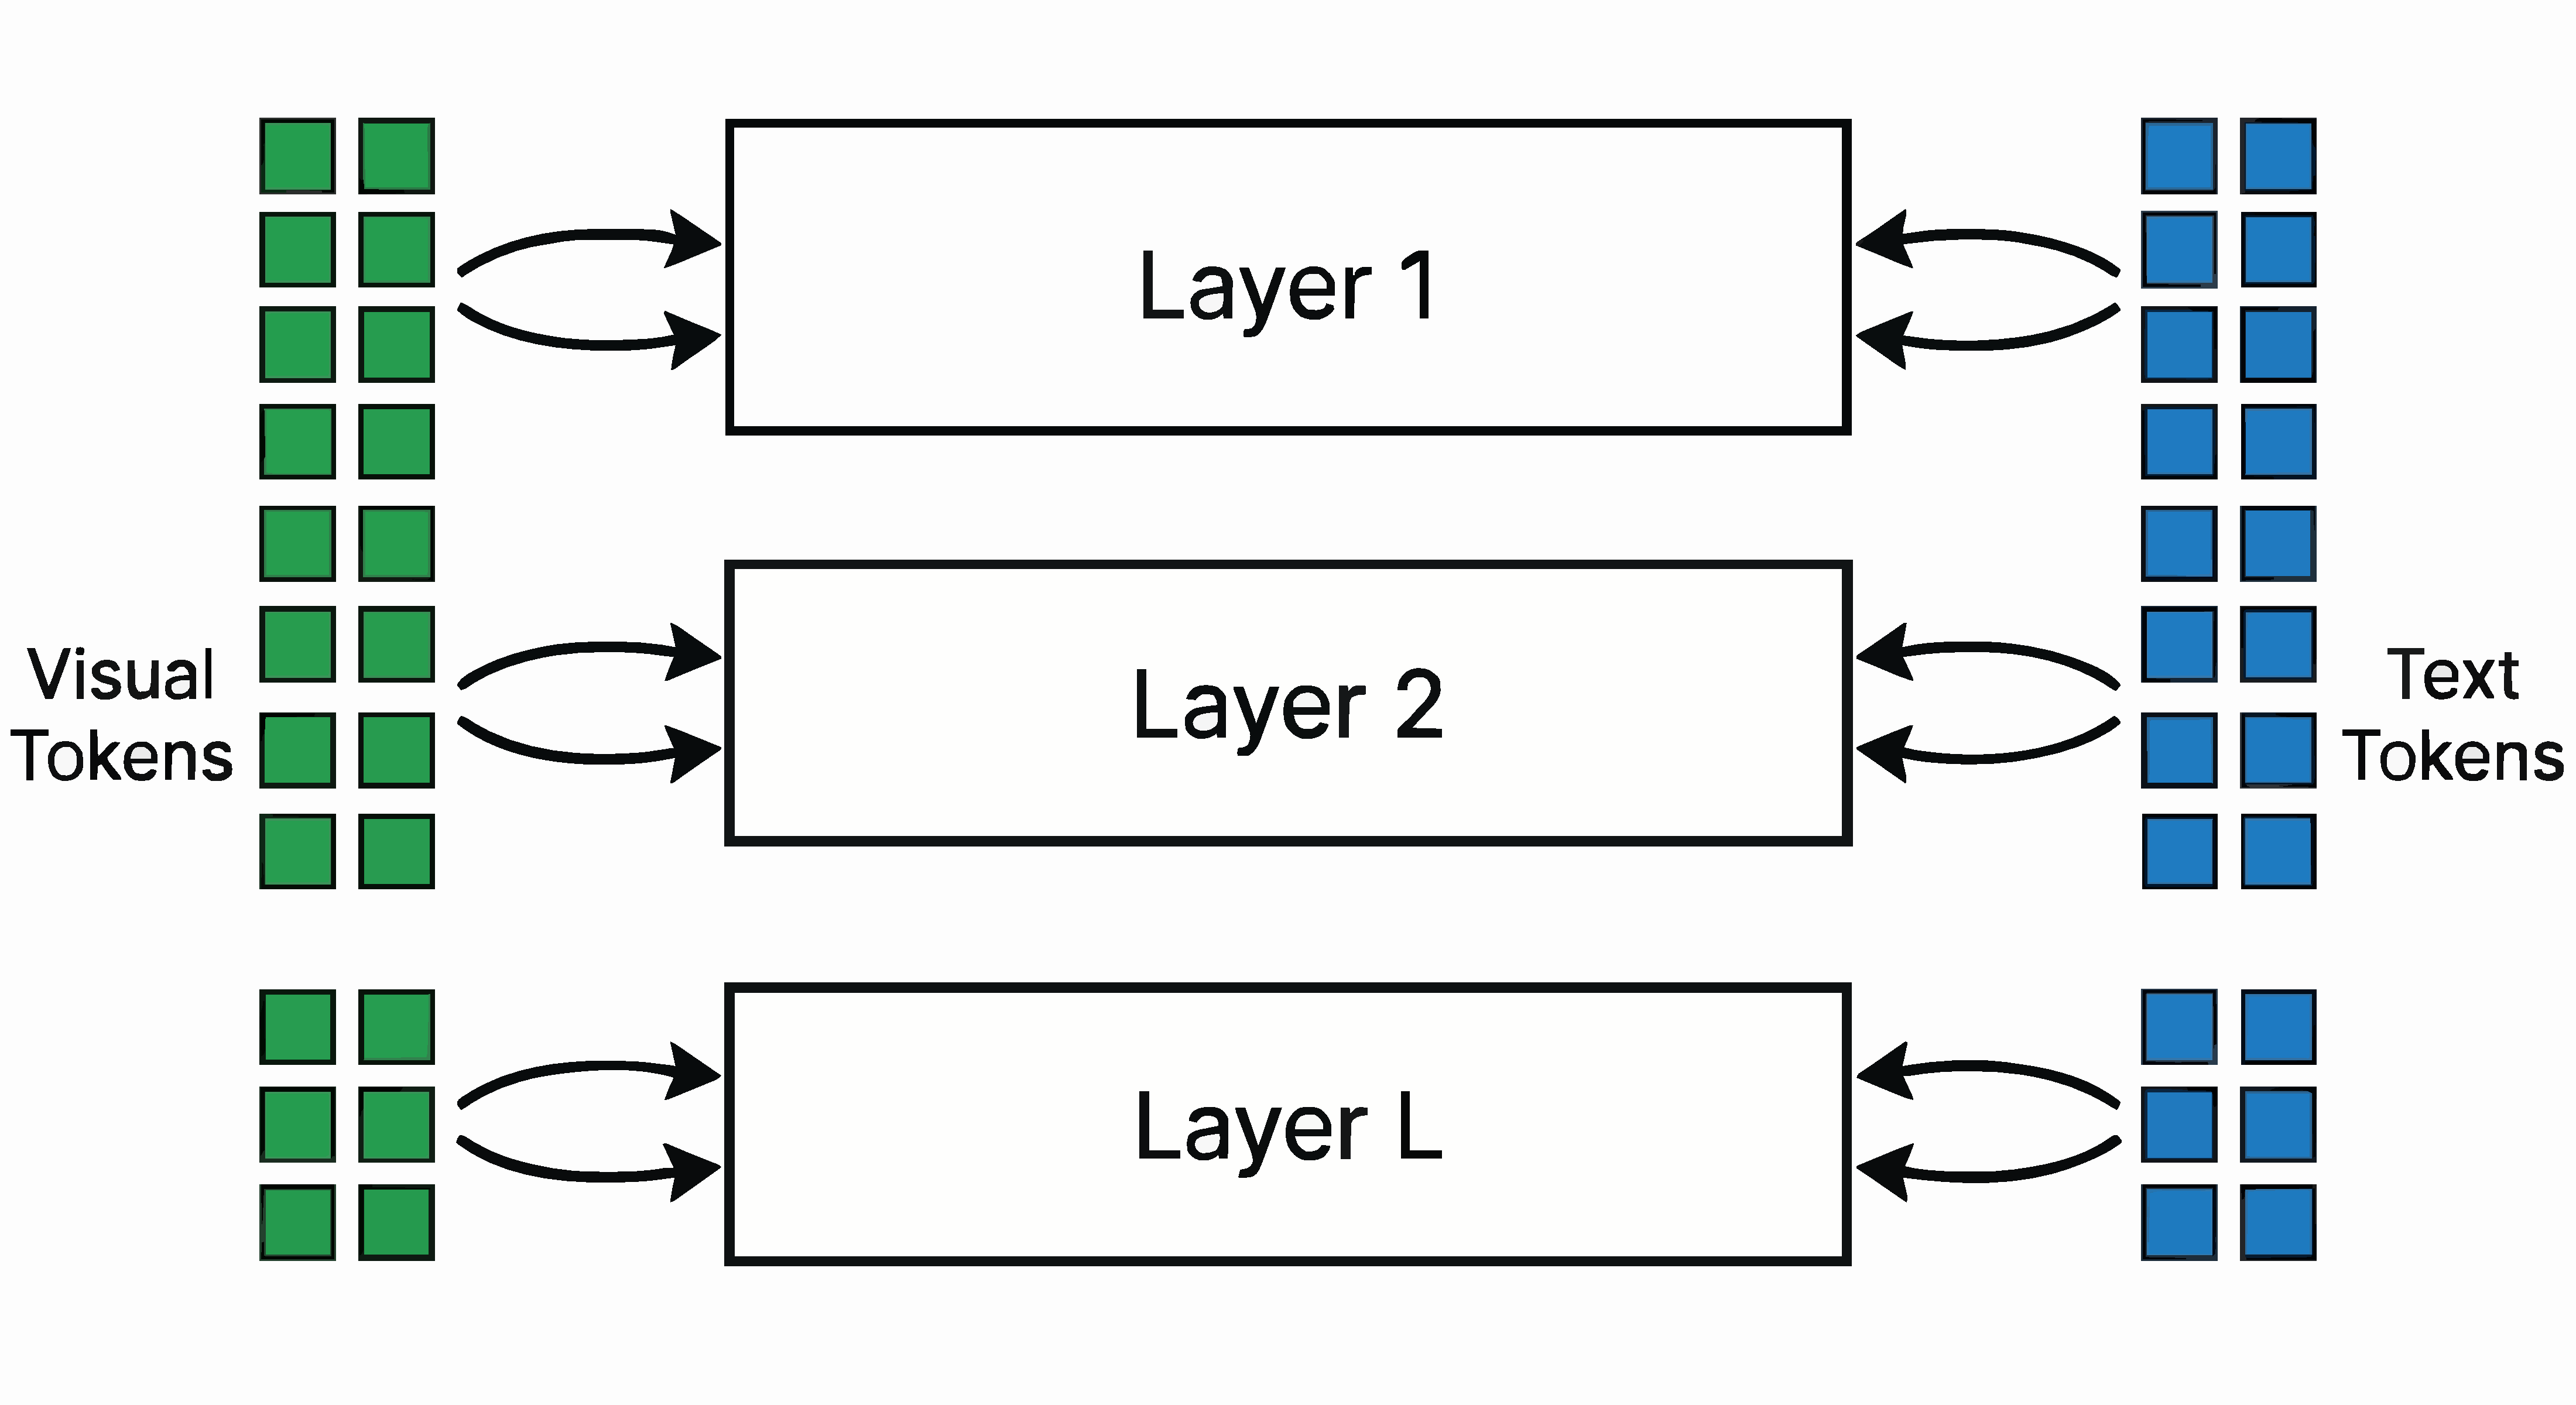
\includegraphics[width=\linewidth]{figs/fig3_alignment}
  \caption{多模态思维链的多维对齐与演进机制图（自绘）。离散视觉 Token 与文本 Token 在统一 Transformer 各层（Layer）内共享潜在空间并实现跨模态双向联合演进。}\label{fig:align}
\end{figure}

% =====================================================================
\section{主要方法的定量对比分析}\label{sec:comparison}
\begin{table}[htbp]
  \centering
  \caption{多模态思维链主要方法在 ScienceQA 上的定量对比（原创整理）}\label{tab:compare}
  \footnotesize
  \resizebox{\linewidth}{!}{%
  \begin{tabularx}{\linewidth}{lYYYY}
    \toprule
    方法 & 架构范式 & 视觉表征 & 阶段数 & 准确率/\% \\
    \midrule
    GPT-4(CoT)     & 单阶段端到端 & 连续     & 1 & 83.99 \\
    LLaVA          & 单阶段端到端 & 连续     & 1 & 90.92 \\
    两阶段解耦     & 两阶段解耦   & 连续     & 2 & 91.68 \\
    Chameleon      & 交织生成     & 离散     & 1 & 86.04 \\
    VLM-R$^3$      & 工具驱动     & 连续+裁剪 & 多 & 92.1 \\
    Visual Planning& 原生视觉想象 & 离散     & 多 & -- \\
    \bottomrule
  \end{tabularx}%
  }
\end{table}
对表~\ref{tab:compare} 所汇总的定量结果加以审视，可归纳出三条并非自明的影响规律。其一，架构范式的解耦程度与推理稳定性之间存在非线性关联：两阶段解耦框架虽引入阶段间信息瓶颈，却因对理由生成与答案预测施加分别监督，在 ScienceQA 上将平均准确率推至 91.68\%，反超单阶段端到端的 LLaVA（90.92\%）；然而同为单阶段的 GPT-4（CoT）仅得 83.99\%，表明单阶段范式对模型容量与预训练先验的依赖远甚于两阶段，小模型在缺乏强先验时贸然采用端到端交织反而易引发跨模态语义漂移。其二，视觉表征的离散性并非性能的充要条件：Chameleon 以离散词元进行交织生成，却仅获 86.04\%，落后于采用连续表征的 LLaVA 达 4.88 个百分点，印证第~\ref{sec:vt:contdisc} 节之论断——离散化不可避免地引入了量化噪声，在码本容量与因果性未充分调优时其代价可能盖过可溯源收益。其三，推理阶段数与准确率呈弱正相关但伴随边际递减：VLM-R$^{3}$ 以多阶段工具驱动达到 92.1\% 的当前最优，其增益主要源自裁剪操作对关键证据的聚焦而非阶段数本身，盲目堆叠阶段而无证据引导只会放大误差累积。需指出的是，Visual Planning 因评测协议差异尚缺可比准确率，其以纯图像思考所牺牲的语言锚点是否会令其在需符号演算的任务上表征坍塌，仍有待基准补全后方能定论。综上，性能差异的本质不在于"离散优于连续"或"多阶段优于单阶段"的二元判断，而在于表征分辨率、监督粒度与证据聚焦三者间的权衡是否与模型容量及任务特性相匹配。


% =====================================================================
\section{研究挑战与未来方向}\label{sec:challenge}

\subsection{逻辑幻觉的级联放大与显式阻断机制}\label{sec:ch:hallu}
视觉幻觉（“看错”）已为事后特征验证流派（Woodpecker）所部分抑制，然逻辑幻觉（Logical Hallucination）——即推理链中公式误用、前后矛盾、推理断层等逻辑谬误——在跨模态协同中呈现出较视觉幻觉更为隐蔽且更具破坏性的级联放大特性。在两阶段解耦框架中，阶段一生成的理由 $r$ 若含逻辑谬误，将以 $P_{\theta_{2}}(a\mid I,Q,r)$ 的条件结构向最终答案传递，谬误随推理步数 $t$ 近似指数累积，终至“一本正经的胡说八道”。现有 Self-Refine、Self-Review 与 Self-Choose 等动态反思机制虽能缓解单一谬误，然其多依赖单一判别器，缺乏对逻辑谬误类型的细粒度识别，且反思本身亦不可避免地引入了噪声。未来宜构建显式逻辑阻断机制：其一，于推理链关键节点引入因果干预（causal intervention）进行反事实检验——若移除某步理由 $r_{t}$ 后答案分布不变，则判定该步为冗余或谬误节点予以剪除，形式化地表为阻断指标：
\begin{multline}\label{eq:cf}
\Delta_{t}=\mathrm{KL}\!\bigl(P_{\theta}(a\mid I,Q,\mathbf{r})\;\big\|\;P_{\theta}(a\mid I,Q,\mathbf{r}_{\setminus t})\bigr), \\
\text{若}\;\Delta_{t}<\tau\;\text{则剪除}\;r_{t}
\end{multline}
其中 $\mathbf{r}_{\setminus t}$ 表示移除第 $t$ 步理由后的推理链，$\tau$ 为显著性阈值，$\mathrm{KL}$ 为 KL 散度；其二，部署针对算术谬误、空间关系谬误与时序因果谬误的多判别器集成（ensemble），实现谬误类型的精准定位与定向阻断；其三，将 GRPO 等强化学习的奖励信号自“最终答案正确性”前移至“每步推理的逻辑一致性”，使阻断内化为模型自身的推理习惯而非事后补丁。

\subsection{细粒度视觉词元的动态按需解耦与语义重构}\label{sec:ch:decouple}
当前视觉词元化普遍采用固定粒度的 patch 或固定码本，在多目标、遮挡、小目标密集等复杂场景下面临表征分辨率与计算开销的两难：粗粒度 token 丢失边界与小目标细节，细粒度 token 则令序列过长而引发 $O(N^{2})$ 自注意力开销的爆炸。DynamicViT 的渐进剪枝与 ToMe 的二分图匹配合并虽提供了稀疏化思路，然二者均为离线、与任务无关的静态压缩，无法随推理难度自适应调节，信息瓶颈受限于预设的压缩比例。未来需实现动态按需解耦（Dynamic Decoupling）：其一，令模型依据问题难度自适应调节词元分辨率——简单问题直接以粗粒度 token 作答，复杂问题则按需调用树搜索对关键区域细粒度重采样，使计算预算向关键证据倾斜；其二，构建可学习的语义重构码本，使码本向量在训练中依据下游推理任务反馈动态演化，而非固着于重建目标；其三，探索层次化词元树（token tree），底层 token 承载细节、高层 token 承载语义，推理时按需激活相应层级，于表征力与效率间取得动态平衡，避免一味追求细粒度而妥协于硬件开销。

\subsection{资源受限环境下的轻量化思维链自适应剪枝}\label{sec:ch:prune}
多模态思维链的多步推理与多模态融合带来高昂计算开销，而具身智能与边缘部署要求模型于毫瓦级功耗下实时推理。现有轻量化手段（量化、蒸馏）多面向模型参数，鲜有针对推理链本身的结构性剪枝。Visual Planning 所提“按需自适应思考”已初现端倪，然尚未系统化。未来应发展自适应思维链剪枝（Adaptive CoT Pruning）：其一，训练一轻量难度评估器预测问题所需的最小推理步数 $T^{*}$，对简单问题直接跳过中间理由生成以走“思考捷径”，对难题方展开完整链；其二，将词元剪枝与推理步剪枝联合优化——不仅剪除冗余视觉 token，更剪除对最终答案边际贡献低于阈值的推理步，使推理链长度随难度弹性伸缩；其三，面向边缘硬件设计混合精度思维链，关键证据步采用高精度离散 token、非关键步降级为低精度连续特征，于精度-延迟曲线上寻求帕累托最优，而非在精度与效率间作非此即彼的零和取舍。

\subsection{面向物理世界交互的具身闭环动态思维链演进}\label{sec:ch:embodied}
当前多模态思维链多在静态图像上进行单向推演，缺乏与物理环境的闭环交互。CoT-VLA\cite{zhao2025cotvla} 与 FutureSightDrive\cite{zhang2025fsd} 虽已将视觉想象引入具身场景，然仍局限于“预测—执行”的开环结构，未实现“执行—观测—修正”的闭环演进。未来应构建具身闭环动态思维链：其一，将物理世界反馈（机器人本体传感器、车载摄像头）作为思维链的实时观测输入，使推理链随环境状态动态修正——当预测的未来帧与实际观测不符时触发 Self-Refine 式的链回溯与重规划；其二，引入世界模型（world model）作为思维链的内部模拟器，于执行前在潜在空间多次推演候选动作的物理后果并择优执行，将“思考”自符号推演扩展为物理因果模拟；其三，建立长周期记忆与思维链的耦合，使具身智能体跨任务积累的物理常识沉淀为推理先验，实现自单次任务推理向终身具身认知的跃迁。此一方向是模式识别自静态旁观迈向动态干预、重塑人机边界的终极形态，亦是对本文所论“感知—推理深度闭环”主线的自然收束。

% =====================================================================
\section{结论}\label{sec:conclusion}
本文以“开放词汇感知提供空间语义奠基 $\rightarrow$ 视觉词元化将图像转化为离散序列 $\rightarrow$ 统一 Transformer 实现多模态思维链动态演进”之层次逻辑为主线，系统梳理了多模态思维链推理自文本 CoT 至具身闭环演进的研究脉络。研究表明，连续特征在多步推理中因注意力稀释而易于失忆，离散视觉词元虽以量化噪声为代价却提供了可溯源的中间状态；两阶段解耦与单阶段交织的取舍并非二元优劣，而取决于表征分辨率、监督粒度与证据聚焦三者之权衡是否匹配模型容量与任务特性。三者层级支撑具有不可逆性，任一环节的妥协均沿因果链向下游传导为不可逆之性能衰减。展望未来，逻辑幻觉的级联阻断、细粒度词元的动态解耦、轻量化自适应剪枝与具身闭环演进构成四个亟待突破的深度方向，其共同指向“感知—推理深度闭环、内生能力与外脑增强融合”的可信赖多模态认知范式。需申明的是，本文所述技术脉络尚处快速演进之中，诸多结论将随基准与模型的迭代而被重新校验，然其层级协同的逻辑框架或可为后续研究提供相对稳定的参照坐标。

% ---------------- 致谢 ----------------
\section*{致\quad 谢}
感谢老师和助教师兄在模式识别课程学习中的付出。
% ---------------- 参考文献 ----------------
\begin{thebibliography}{99}
\bibitem{wei2022cot} Wei J, Wang X, Schuurmans D, et al. Chain-of-thought prompting elicits reasoning in large language models. Advances in Neural Information Processing Systems, 2022, 35: 24824-24837
\bibitem{zhang2023mcot} Zhang Z, Zhang A, Li M, et al. Multimodal chain-of-thought reasoning in language models. Transactions on Machine Learning Research, 2023
\bibitem{radford2021clip} Radford A, Kim J W, Hallacy C, et al. Learning transferable visual models from natural language supervision. //Proceedings of the International Conference on Machine Learning. PMLR, 2021: 8748-8763
\bibitem{li2022gllip} Li L H, Zhang P, Zhang H, et al. Grounded language-image pre-training. //Proceedings of the IEEE/CVF Conference on Computer Vision and Pattern Recognition. New Orleans, USA, 2022: 10965-10975
\bibitem{liu2024groundingdino} Liu S, Zeng Z, Ren T, et al. Grounding DINO: Marrying DINO with grounded pre-training for open-set object detection. //Proceedings of the European Conference on Computer Vision. Milan, Italy, 2024
\bibitem{li2023lisa} Lai X, Tian Z, Chen Y, et al. LISA: Reasoning segmentation via large language models. arXiv preprint arXiv:2308.00692, 2023
\bibitem{van2017vqvae} van den Oord A, Vinyals O, Kavukcuoglu K. Neural discrete representation learning. Advances in Neural Information Processing Systems, 2017, 30
\bibitem{ge2023seed} Ge Y, Song Y, Zhang C, et al. Planting a SEED of vision in large language model. arXiv preprint arXiv:2307.08041, 2023
\bibitem{liu2024univl} Liu H, Li C, Wu Q, et al. Visual instruction tuning. Advances in Neural Information Processing Systems, 2024, 36
\bibitem{team2024chameleon} Chameleon Team. Chameleon: Mixed-modal early-fusion foundation models. arXiv preprint arXiv:2405.09818, 2024
\bibitem{xu2026visualplanning} Xu Y, et al. Visual planning: Let's think only with images. //Proceedings of ICLR, 2026
\bibitem{zhao2025cotvla} Zhao Q, et al. CoT-VLA: Visual chain-of-thought reasoning for vision-language-action models. //Proceedings of CVPR, 2025
\bibitem{esser2021vqgan} Esser P, Rombach R, Ommer B. Taming transformers for high-resolution image synthesis. //Proceedings of the IEEE/CVF Conference on Computer Vision and Pattern Recognition. Virtual, 2021: 12873-12883
\bibitem{fei2025unitok} Fei X, et al. UniTok: A unified tokenizer for visual generation and understanding. //Proceedings of NeurIPS, 2025
\bibitem{zhang2025fsd} Zhang S, et al. FutureSightDrive: Thinking visually with spatio-temporal CoT for autonomous driving. //Proceedings of NeurIPS, 2025
\end{thebibliography}

\balance
\end{document}

